\documentclass[aspectratio=169]{beamer}

% Minimal theme
\usetheme{default}
\usecolortheme{dove}

% Remove navigation symbols
\setbeamertemplate{navigation symbols}{}
\setbeamertemplate{footline}{%
  \hfill{\large\insertframenumber\,/\,\inserttotalframenumber}\hspace{0.8em}\vspace{0.5em}%
}

% Colors
\definecolor{popblue}{RGB}{52, 101, 164}
\definecolor{sampred}{RGB}{204, 0, 0}
\definecolor{paramgreen}{RGB}{0, 140, 70}
\definecolor{lightbg}{RGB}{245, 245, 250}
\definecolor{warnred}{RGB}{180, 40, 40}
\definecolor{orange1}{RGB}{220, 120, 0}
\definecolor{violet1}{RGB}{120, 50, 160}

\setbeamercolor{frametitle}{fg=popblue}
\setbeamercolor{title}{fg=popblue}

% Packages
\usepackage{pgfplots}
\usepackage{tikz}
\usetikzlibrary{shapes, arrows.meta, positioning, calc, decorations.pathreplacing, patterns, fit}
\pgfplotsset{compat=1.18}
\usepackage{amsmath, amssymb}
\usepackage{array}
\usepackage{fontenc}

\title{AI Agents \& Tool Use}
\subtitle{ReAct $\cdot$ Function Calling $\cdot$ Multi-Agent $\cdot$ MCP}
\date{}

\begin{document}

% ============================================================
% TITLE
% ============================================================
\begin{frame}
\titlepage
\end{frame}

% ============================================================
% WHAT IS AN AI AGENT?
% ============================================================
\begin{frame}
\frametitle{What is an AI agent?}

\begin{center}
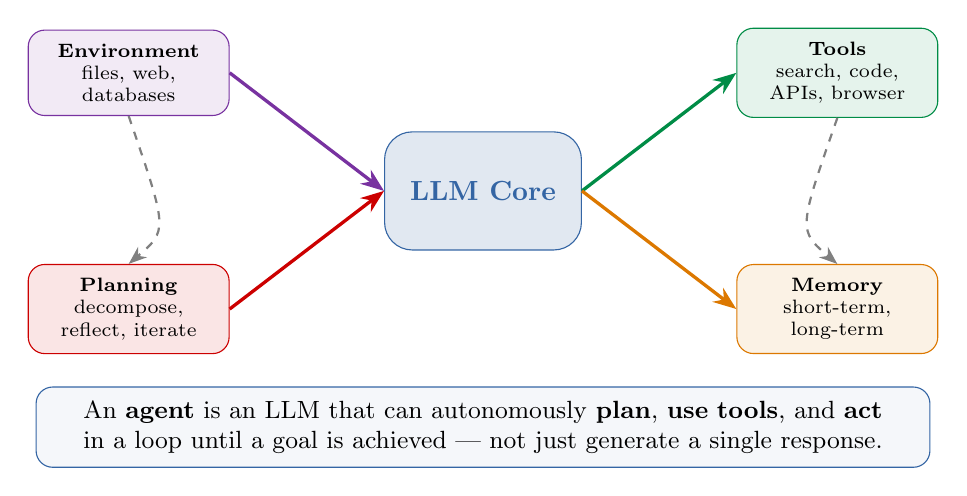
\begin{tikzpicture}
  % Central LLM
  \node[draw=popblue, fill=popblue!15, rounded corners=10pt, minimum width=2.5cm, minimum height=1.5cm, font=\normalsize\bfseries, text=popblue] (llm) at (0, 0) {LLM Core};

  % Tools
  \node[draw=paramgreen, fill=paramgreen!10, rounded corners=6pt, text width=2.2cm, align=center, inner sep=5pt, font=\scriptsize] (tools) at (4.5, 1.5) {\textbf{Tools}\\search, code,\\APIs, browser};
  \draw[-Stealth, very thick, paramgreen] (llm.east) -- (tools.west);

  % Memory
  \node[draw=orange1, fill=orange1!10, rounded corners=6pt, text width=2.2cm, align=center, inner sep=5pt, font=\scriptsize] (mem) at (4.5, -1.5) {\textbf{Memory}\\short-term,\\long-term};
  \draw[-Stealth, very thick, orange1] (llm.east) -- (mem.west);

  % Environment
  \node[draw=violet1, fill=violet1!10, rounded corners=6pt, text width=2.2cm, align=center, inner sep=5pt, font=\scriptsize] (env) at (-4.5, 1.5) {\textbf{Environment}\\files, web,\\databases};
  \draw[-Stealth, very thick, violet1] (env.east) -- (llm.west);

  % Planning loop
  \node[draw=sampred, fill=sampred!10, rounded corners=6pt, text width=2.2cm, align=center, inner sep=5pt, font=\scriptsize] (plan) at (-4.5, -1.5) {\textbf{Planning}\\decompose,\\reflect, iterate};
  \draw[-Stealth, very thick, sampred] (plan.east) -- (llm.west);

  % Loop arrow
  \draw[-Stealth, thick, gray, dashed] (tools.south) .. controls (4, -0.5) and (4, -0.5) .. (mem.north);
  \draw[-Stealth, thick, gray, dashed] (env.south) .. controls (-4, -0.5) and (-4, -0.5) .. (plan.north);

  % Bottom
  \node[draw=popblue, fill=popblue!5, rounded corners=6pt, text width=11cm, align=center, inner sep=5pt, font=\small] at (0, -3) {
    An \textbf{agent} is an LLM that can autonomously \textbf{plan}, \textbf{use tools}, and \textbf{act}\\
    in a loop until a goal is achieved --- not just generate a single response.
  };
\end{tikzpicture}
\end{center}
\end{frame}

% ============================================================
% CHATBOT VS AGENT
% ============================================================
\begin{frame}
\frametitle{Chatbot vs.\ agent}

\begin{center}
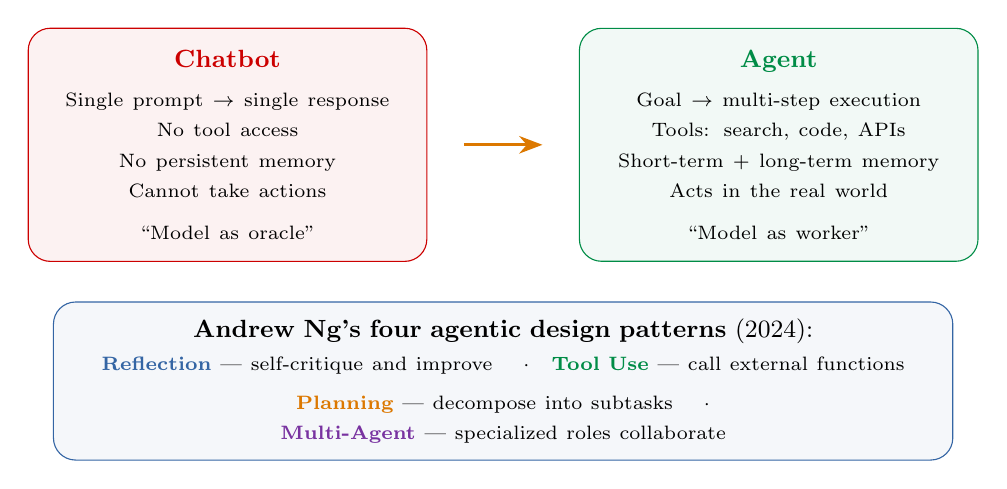
\begin{tikzpicture}
  % Chatbot
  \node[draw=sampred, fill=sampred!5, rounded corners=8pt, text width=4.5cm, align=center, inner sep=8pt] at (-3.5, 1.5) {
    {\small\bfseries\textcolor{sampred}{Chatbot}}\\[6pt]
    {\scriptsize Single prompt $\to$ single response\\[3pt]
    No tool access\\[3pt]
    No persistent memory\\[3pt]
    Cannot take actions\\[3pt]
    ``Model as oracle''}
  };

  % Arrow
  \draw[-Stealth, very thick, orange1] (-0.5, 1.5) -- (0.5, 1.5);

  % Agent
  \node[draw=paramgreen, fill=paramgreen!5, rounded corners=8pt, text width=4.5cm, align=center, inner sep=8pt] at (3.5, 1.5) {
    {\small\bfseries\textcolor{paramgreen}{Agent}}\\[6pt]
    {\scriptsize Goal $\to$ multi-step execution\\[3pt]
    Tools: search, code, APIs\\[3pt]
    Short-term + long-term memory\\[3pt]
    Acts in the real world\\[3pt]
    ``Model as worker''}
  };

  % Ng's patterns
  \node[draw=popblue, fill=popblue!5, rounded corners=8pt, text width=11cm, align=center, inner sep=6pt, font=\small] at (0, -1.5) {
    \textbf{Andrew Ng's four agentic design patterns} (2024):\\[4pt]
    {\scriptsize
    \textcolor{popblue}{\bfseries Reflection} --- self-critique and improve \quad$\cdot$\quad
    \textcolor{paramgreen}{\bfseries Tool Use} --- call external functions\\[3pt]
    \textcolor{orange1}{\bfseries Planning} --- decompose into subtasks \quad$\cdot$\quad
    \textcolor{violet1}{\bfseries Multi-Agent} --- specialized roles collaborate}
  };
\end{tikzpicture}
\end{center}
\end{frame}

% ============================================================
% REACT: REASONING + ACTING
% ============================================================
\begin{frame}
\frametitle{ReAct: Reasoning + Acting}

\begin{center}
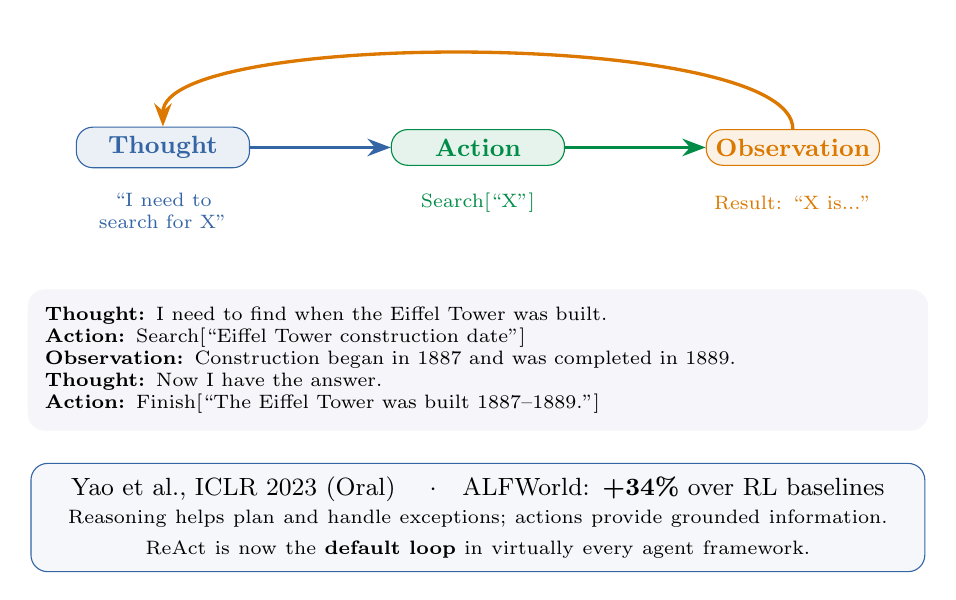
\begin{tikzpicture}
  % Loop
  \node[draw=popblue, fill=popblue!10, rounded corners=6pt, font=\small\bfseries, minimum width=2.2cm, text=popblue] (thought) at (-4, 2.5) {Thought};
  \node[draw=paramgreen, fill=paramgreen!10, rounded corners=6pt, font=\small\bfseries, minimum width=2.2cm, text=paramgreen] (action) at (0, 2.5) {Action};
  \node[draw=orange1, fill=orange1!10, rounded corners=6pt, font=\small\bfseries, minimum width=2.2cm, text=orange1] (obs) at (4, 2.5) {Observation};

  \draw[-Stealth, very thick, popblue] (thought) -- (action);
  \draw[-Stealth, very thick, paramgreen] (action) -- (obs);
  \draw[-Stealth, very thick, orange1] (obs) .. controls (4, 4) and (-4, 4) .. (thought);

  % Labels
  \node[font=\scriptsize, text=popblue, text width=2.5cm, align=center] at (-4, 1.7) {``I need to search for X''};
  \node[font=\scriptsize, text=paramgreen] at (0, 1.8) {Search[``X'']};
  \node[font=\scriptsize, text=orange1] at (4, 1.8) {Result: ``X is...''};

  % Example
  \node[draw=lightbg, fill=lightbg, rounded corners=6pt, text width=11cm, align=left, inner sep=6pt, font=\scriptsize] at (0, -0.2) {
    \textbf{Thought:} I need to find when the Eiffel Tower was built.\\
    \textbf{Action:} Search[``Eiffel Tower construction date'']\\
    \textbf{Observation:} Construction began in 1887 and was completed in 1889.\\
    \textbf{Thought:} Now I have the answer.\\
    \textbf{Action:} Finish[``The Eiffel Tower was built 1887--1889.'']
  };

  % Results
  \node[draw=popblue, fill=popblue!5, rounded corners=6pt, text width=11cm, align=center, inner sep=5pt, font=\small] at (0, -2.2) {
    Yao et al., ICLR 2023 (Oral) \quad$\cdot$\quad ALFWorld: \textbf{+34\%} over RL baselines\\[2pt]
    {\scriptsize Reasoning helps plan and handle exceptions; actions provide grounded information.\\
    ReAct is now the \textbf{default loop} in virtually every agent framework.}
  };
\end{tikzpicture}
\end{center}
\end{frame}

% ============================================================
% FUNCTION CALLING / TOOL USE
% ============================================================
\begin{frame}
\frametitle{Function calling}
\vspace{-0.2cm}
\begin{center}
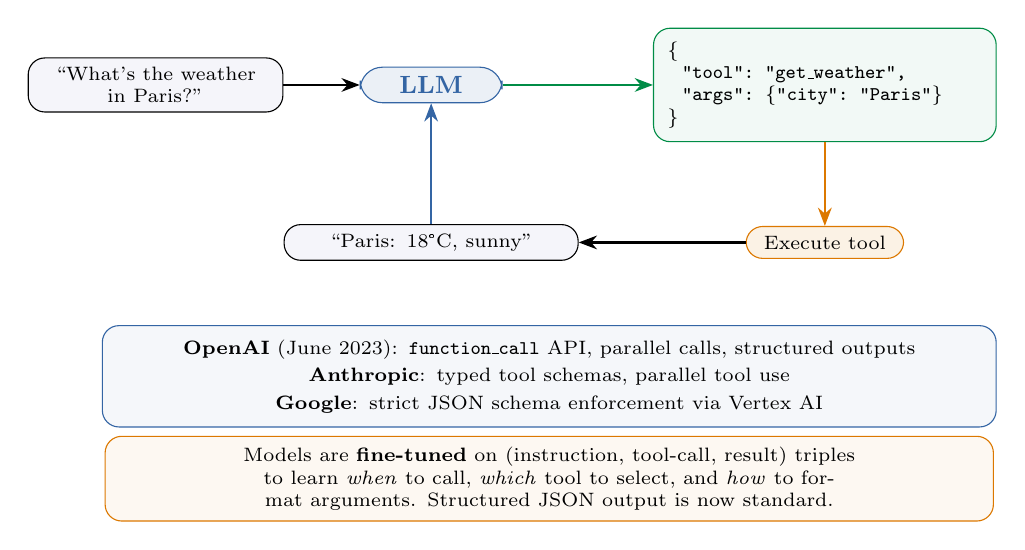
\begin{tikzpicture}
  % User prompt
  \node[draw, rounded corners=6pt, fill=lightbg, font=\scriptsize, text width=3cm, align=center] (user) at (-5, 2.5) {``What's the weather\\in Paris?''};

  % LLM
  \node[draw=popblue, fill=popblue!10, rounded corners=8pt, font=\small\bfseries, text=popblue, minimum width=1.8cm] (llm) at (-1.5, 2.5) {LLM};
  \draw[-Stealth, thick] (user) -- (llm);

  % JSON output
  \node[draw=paramgreen, fill=paramgreen!5, rounded corners=6pt, font=\scriptsize, text width=4cm, align=left, inner sep=5pt] (json) at (3.5, 2.5) {
    \texttt{\{}\\
    \texttt{~~"tool": "get\_weather",}\\
    \texttt{~~"args": \{"city": "Paris"\}}\\
    \texttt{\}}
  };
  \draw[-Stealth, thick, paramgreen] (llm) -- (json);

  % Tool execution
  \node[draw=orange1, fill=orange1!10, rounded corners=6pt, font=\scriptsize, minimum width=2cm] (exec) at (3.5, 0.5) {Execute tool};
  \draw[-Stealth, thick, orange1] (json) -- (exec);

  % Result back
  \node[draw, rounded corners=6pt, fill=lightbg, font=\scriptsize, text width=3.5cm, align=center] (result) at (-1.5, 0.5) {``Paris: 18\textdegree C, sunny''};
  \draw[-Stealth, thick] (exec) -- (result);
  \draw[-Stealth, thick, popblue] (result) -- (llm);

  % Provider comparison
  \node[draw=popblue, fill=popblue!5, rounded corners=6pt, text width=11cm, align=center, inner sep=5pt, font=\scriptsize] at (0, -1.2) {
    \textbf{OpenAI} (June 2023): \texttt{function\_call} API, parallel calls, structured outputs\\[2pt]
    \textbf{Anthropic}: typed tool schemas, parallel tool use\\[2pt]
    \textbf{Google}: strict JSON schema enforcement via Vertex AI
  };

  % Key
  \node[draw=orange1, fill=orange1!5, rounded corners=6pt, text width=11cm, align=center, inner sep=4pt, font=\scriptsize] at (0, -2.5) {
    Models are \textbf{fine-tuned} on (instruction, tool-call, result) triples to learn \textit{when} to call,
    \textit{which} tool to select, and \textit{how} to format arguments. Structured JSON output is now standard.
  };
\end{tikzpicture}
\end{center}
\end{frame}

% ============================================================
% TYPES OF TOOLS
% ============================================================
\begin{frame}
\frametitle{Types of tools}

\begin{center}
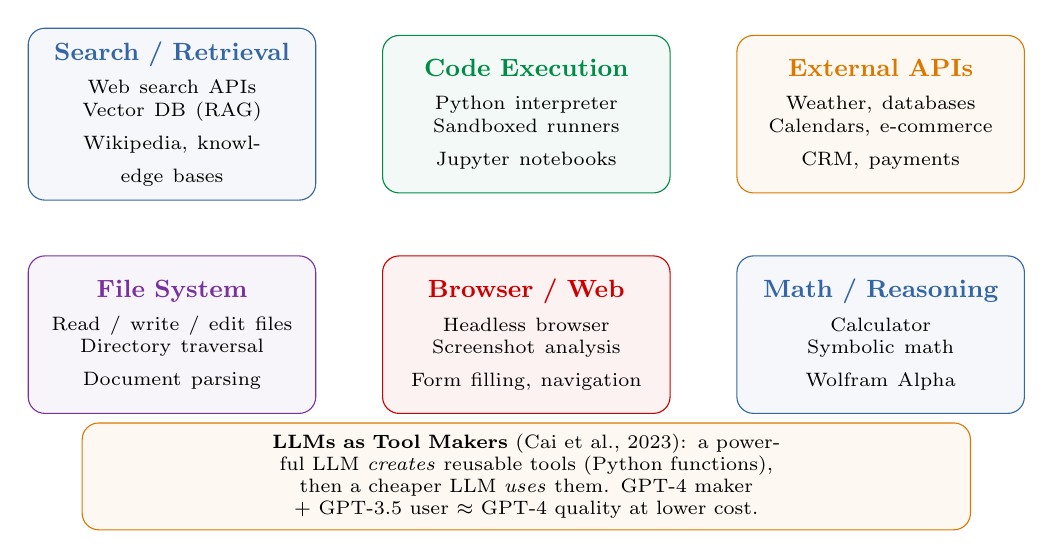
\begin{tikzpicture}
  % Tool cards - row 1
  \node[draw=popblue, fill=popblue!5, rounded corners=6pt, text width=3.3cm, align=center, inner sep=5pt, minimum height=2cm] at (-4.5, 2) {
    {\small\bfseries\textcolor{popblue}{Search / Retrieval}}\\[4pt]
    {\scriptsize Web search APIs\\
    Vector DB (RAG)\\
    Wikipedia, knowledge bases}
  };

  \node[draw=paramgreen, fill=paramgreen!5, rounded corners=6pt, text width=3.3cm, align=center, inner sep=5pt, minimum height=2cm] at (0, 2) {
    {\small\bfseries\textcolor{paramgreen}{Code Execution}}\\[4pt]
    {\scriptsize Python interpreter\\
    Sandboxed runners\\
    Jupyter notebooks}
  };

  \node[draw=orange1, fill=orange1!5, rounded corners=6pt, text width=3.3cm, align=center, inner sep=5pt, minimum height=2cm] at (4.5, 2) {
    {\small\bfseries\textcolor{orange1}{External APIs}}\\[4pt]
    {\scriptsize Weather, databases\\
    Calendars, e-commerce\\
    CRM, payments}
  };

  % Row 2
  \node[draw=violet1, fill=violet1!5, rounded corners=6pt, text width=3.3cm, align=center, inner sep=5pt, minimum height=2cm] at (-4.5, -0.8) {
    {\small\bfseries\textcolor{violet1}{File System}}\\[4pt]
    {\scriptsize Read / write / edit files\\
    Directory traversal\\
    Document parsing}
  };

  \node[draw=sampred, fill=sampred!5, rounded corners=6pt, text width=3.3cm, align=center, inner sep=5pt, minimum height=2cm] at (0, -0.8) {
    {\small\bfseries\textcolor{sampred}{Browser / Web}}\\[4pt]
    {\scriptsize Headless browser\\
    Screenshot analysis\\
    Form filling, navigation}
  };

  \node[draw=popblue, fill=popblue!5, rounded corners=6pt, text width=3.3cm, align=center, inner sep=5pt, minimum height=2cm] at (4.5, -0.8) {
    {\small\bfseries\textcolor{popblue}{Math / Reasoning}}\\[4pt]
    {\scriptsize Calculator\\
    Symbolic math\\
    Wolfram Alpha}
  };

  % LATM
  \node[draw=orange1, fill=orange1!5, rounded corners=6pt, text width=11cm, align=center, inner sep=4pt, font=\scriptsize] at (0, -2.6) {
    \textbf{LLMs as Tool Makers} (Cai et al., 2023): a powerful LLM \textit{creates} reusable tools (Python functions),\\
    then a cheaper LLM \textit{uses} them. GPT-4 maker + GPT-3.5 user $\approx$ GPT-4 quality at lower cost.
  };
\end{tikzpicture}
\end{center}
\end{frame}

% ============================================================
% TOOLFORMER
% ============================================================
\begin{frame}
\frametitle{Toolformer: self-supervised tool learning}

\begin{center}
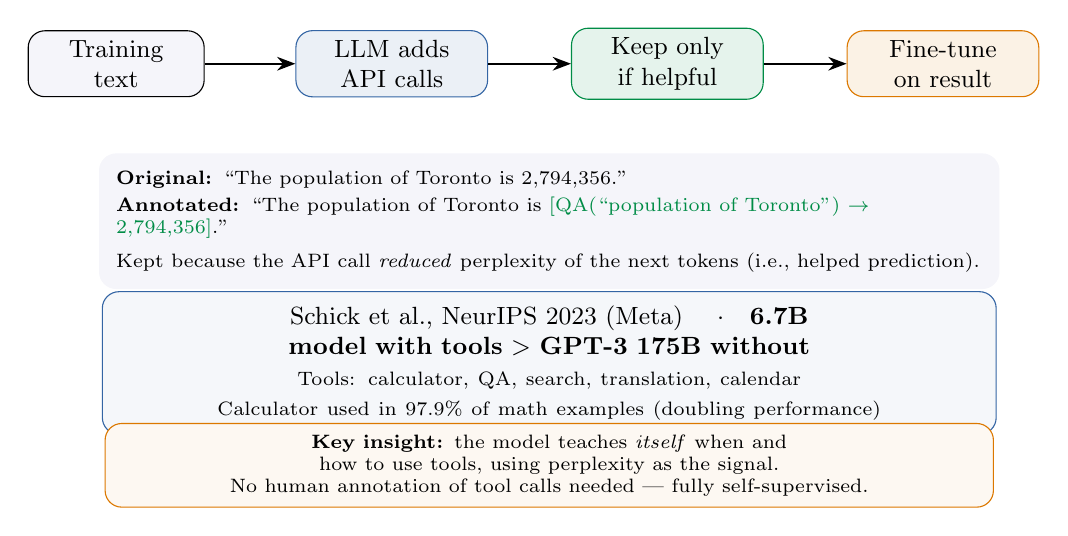
\begin{tikzpicture}
  % Pipeline
  \node[draw, rounded corners=6pt, fill=lightbg, font=\small, text width=2cm, align=center] (text) at (-5.5, 2.5) {Training\\text};
  \node[draw=popblue, fill=popblue!10, rounded corners=6pt, font=\small, text width=2.2cm, align=center] (annotate) at (-2, 2.5) {LLM adds\\API calls};
  \node[draw=paramgreen, fill=paramgreen!10, rounded corners=6pt, font=\small, text width=2.2cm, align=center] (filter) at (1.5, 2.5) {Keep only\\if helpful};
  \node[draw=orange1, fill=orange1!10, rounded corners=6pt, font=\small, text width=2.2cm, align=center] (train) at (5, 2.5) {Fine-tune\\on result};

  \draw[-Stealth, thick] (text) -- (annotate);
  \draw[-Stealth, thick] (annotate) -- (filter);
  \draw[-Stealth, thick] (filter) -- (train);

  % Example
  \node[draw=lightbg, fill=lightbg, rounded corners=6pt, text width=11cm, align=left, inner sep=6pt, font=\scriptsize] at (0, 0.5) {
    \textbf{Original:} ``The population of Toronto is 2,794,356.''\\[2pt]
    \textbf{Annotated:} ``The population of Toronto is \textcolor{paramgreen}{[QA(``population of Toronto'') $\to$ 2,794,356]}.''\\[4pt]
    {\scriptsize Kept because the API call \textit{reduced} perplexity of the next tokens (i.e., helped prediction).}
  };

  % Results
  \node[draw=popblue, fill=popblue!5, rounded corners=6pt, text width=11cm, align=center, inner sep=5pt, font=\small] at (0, -1.3) {
    Schick et al., NeurIPS 2023 (Meta) \quad$\cdot$\quad \textbf{6.7B model with tools $>$ GPT-3 175B without}\\[3pt]
    {\scriptsize Tools: calculator, QA, search, translation, calendar\\
    Calculator used in 97.9\% of math examples (doubling performance)}
  };

  % Key insight
  \node[draw=orange1, fill=orange1!5, rounded corners=6pt, text width=11cm, align=center, inner sep=4pt, font=\scriptsize] at (0, -2.6) {
    \textbf{Key insight:} the model teaches \textit{itself} when and how to use tools, using perplexity as the signal.\\
    No human annotation of tool calls needed --- fully self-supervised.
  };
\end{tikzpicture}
\end{center}
\end{frame}

% ============================================================
% PLANNING & DECOMPOSITION
% ============================================================
\begin{frame}
\frametitle{Planning \& decomposition}

\begin{center}
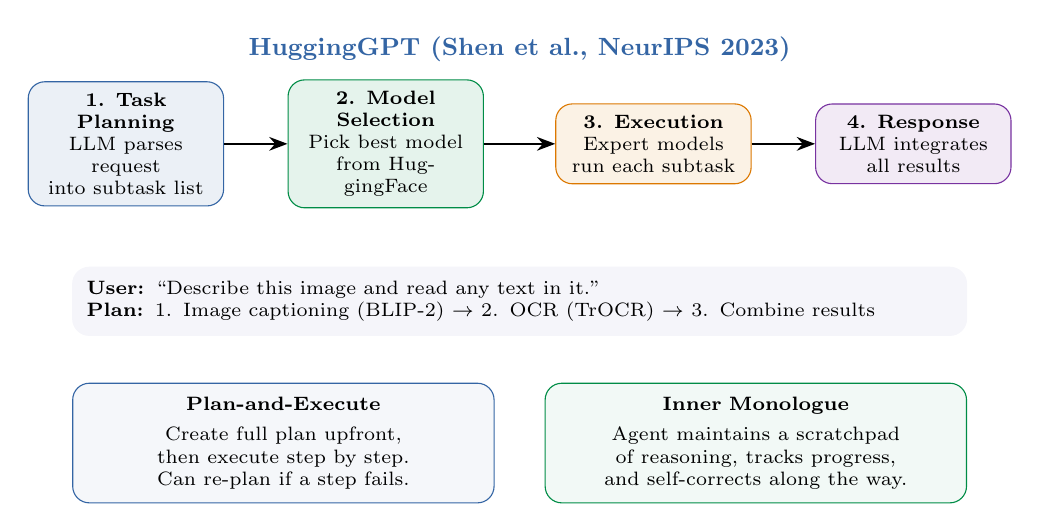
\begin{tikzpicture}
  % HuggingGPT pipeline
  \node[font=\small\bfseries, text=popblue] at (0, 3.2) {HuggingGPT (Shen et al., NeurIPS 2023)};

  \node[draw=popblue, fill=popblue!10, rounded corners=6pt, font=\scriptsize, text width=2.2cm, align=center, inner sep=4pt] (s1) at (-5, 2) {\textbf{1. Task Planning}\\LLM parses request\\into subtask list};
  \node[draw=paramgreen, fill=paramgreen!10, rounded corners=6pt, font=\scriptsize, text width=2.2cm, align=center, inner sep=4pt] (s2) at (-1.7, 2) {\textbf{2. Model Selection}\\Pick best model\\from HuggingFace};
  \node[draw=orange1, fill=orange1!10, rounded corners=6pt, font=\scriptsize, text width=2.2cm, align=center, inner sep=4pt] (s3) at (1.7, 2) {\textbf{3. Execution}\\Expert models\\run each subtask};
  \node[draw=violet1, fill=violet1!10, rounded corners=6pt, font=\scriptsize, text width=2.2cm, align=center, inner sep=4pt] (s4) at (5, 2) {\textbf{4. Response}\\LLM integrates\\all results};

  \draw[-Stealth, thick] (s1) -- (s2);
  \draw[-Stealth, thick] (s2) -- (s3);
  \draw[-Stealth, thick] (s3) -- (s4);

  % Example
  \node[draw=lightbg, fill=lightbg, rounded corners=6pt, text width=11cm, align=left, inner sep=5pt, font=\scriptsize] at (0, 0) {
    \textbf{User:} ``Describe this image and read any text in it.''\\
    \textbf{Plan:} 1. Image captioning (BLIP-2) $\to$ 2. OCR (TrOCR) $\to$ 3. Combine results
  };

  % General patterns
  \node[draw=popblue, fill=popblue!5, rounded corners=6pt, text width=5cm, align=center, inner sep=5pt, font=\scriptsize] at (-3, -1.8) {
    \textbf{Plan-and-Execute}\\[3pt]
    Create full plan upfront,\\
    then execute step by step.\\
    Can re-plan if a step fails.
  };

  \node[draw=paramgreen, fill=paramgreen!5, rounded corners=6pt, text width=5cm, align=center, inner sep=5pt, font=\scriptsize] at (3, -1.8) {
    \textbf{Inner Monologue}\\[3pt]
    Agent maintains a scratchpad\\
    of reasoning, tracks progress,\\
    and self-corrects along the way.
  };
\end{tikzpicture}
\end{center}
\end{frame}

% ============================================================
% MEMORY SYSTEMS
% ============================================================
\begin{frame}
\frametitle{Memory systems}

\begin{center}
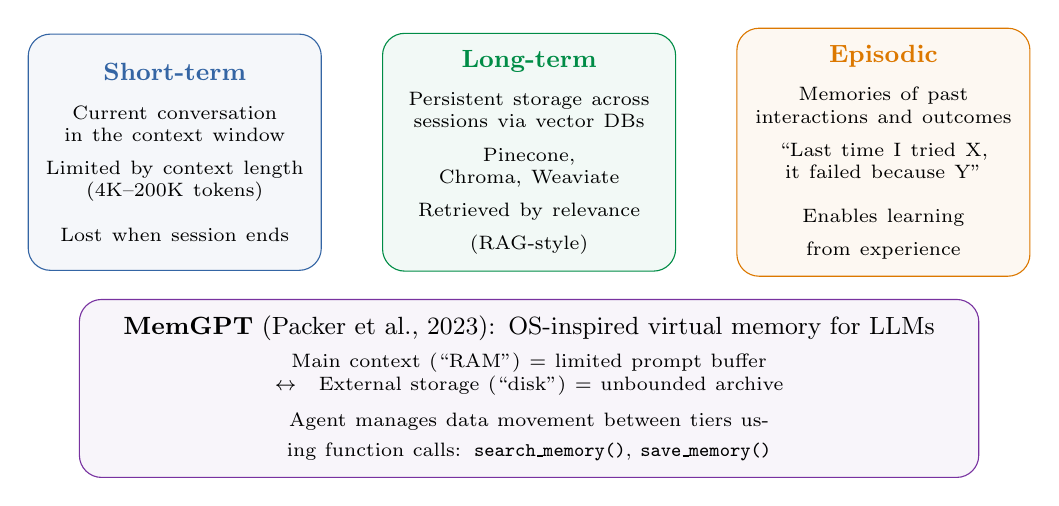
\begin{tikzpicture}
  % Three memory types
  \node[draw=popblue, fill=popblue!5, rounded corners=8pt, text width=3.3cm, align=center, inner sep=6pt, minimum height=3cm] at (-4.5, 1.5) {
    {\small\bfseries\textcolor{popblue}{Short-term}}\\[6pt]
    {\scriptsize Current conversation\\in the context window\\[4pt]
    Limited by context length\\(4K--200K tokens)\\[4pt]
    Lost when session ends}
  };

  \node[draw=paramgreen, fill=paramgreen!5, rounded corners=8pt, text width=3.3cm, align=center, inner sep=6pt, minimum height=3cm] at (0, 1.5) {
    {\small\bfseries\textcolor{paramgreen}{Long-term}}\\[6pt]
    {\scriptsize Persistent storage across\\sessions via vector DBs\\[4pt]
    Pinecone, Chroma, Weaviate\\[4pt]
    Retrieved by relevance\\(RAG-style)}
  };

  \node[draw=orange1, fill=orange1!5, rounded corners=8pt, text width=3.3cm, align=center, inner sep=6pt, minimum height=3cm] at (4.5, 1.5) {
    {\small\bfseries\textcolor{orange1}{Episodic}}\\[6pt]
    {\scriptsize Memories of past\\interactions and outcomes\\[4pt]
    ``Last time I tried X,\\it failed because Y''\\[4pt]
    Enables learning from experience}
  };

  % MemGPT
  \node[draw=violet1, fill=violet1!5, rounded corners=8pt, text width=11cm, align=center, inner sep=6pt, font=\small] at (0, -1.5) {
    \textbf{MemGPT} (Packer et al., 2023): OS-inspired virtual memory for LLMs\\[4pt]
    {\scriptsize Main context (``RAM'') = limited prompt buffer \quad$\leftrightarrow$\quad External storage (``disk'') = unbounded archive\\[2pt]
    Agent manages data movement between tiers using function calls: \texttt{search\_memory()}, \texttt{save\_memory()}}
  };
\end{tikzpicture}
\end{center}
\end{frame}

% ============================================================
% MULTI-AGENT SYSTEMS
% ============================================================
\begin{frame}
\frametitle{Multi-agent systems}

\begin{center}
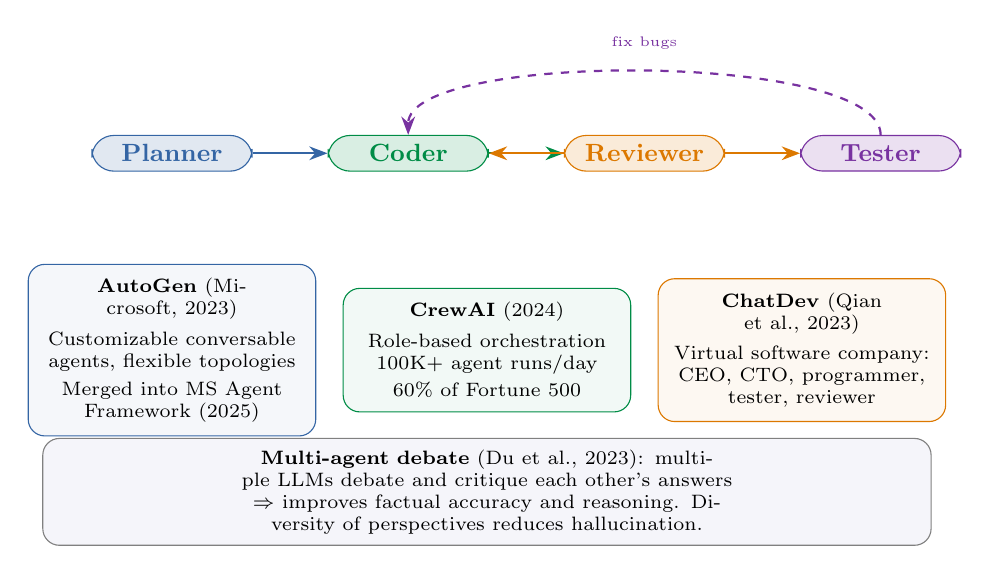
\begin{tikzpicture}
  % Agents
  \node[draw=popblue, fill=popblue!15, rounded corners=8pt, font=\small\bfseries, text width=1.8cm, align=center, text=popblue] (planner) at (-4, 2.5) {Planner};
  \node[draw=paramgreen, fill=paramgreen!15, rounded corners=8pt, font=\small\bfseries, text width=1.8cm, align=center, text=paramgreen] (coder) at (-1, 2.5) {Coder};
  \node[draw=orange1, fill=orange1!15, rounded corners=8pt, font=\small\bfseries, text width=1.8cm, align=center, text=orange1] (reviewer) at (2, 2.5) {Reviewer};
  \node[draw=violet1, fill=violet1!15, rounded corners=8pt, font=\small\bfseries, text width=1.8cm, align=center, text=violet1] (tester) at (5, 2.5) {Tester};

  % Communication arrows
  \draw[-Stealth, thick, popblue] (planner) -- (coder);
  \draw[-Stealth, thick, paramgreen] (coder) -- (reviewer);
  \draw[Stealth-, thick, orange1] (coder) -- (reviewer);
  \draw[-Stealth, thick, orange1] (reviewer) -- (tester);
  \draw[-Stealth, thick, violet1, dashed] (tester) .. controls (5, 3.8) and (-1, 3.8) .. (coder);
  \node[font=\tiny, text=violet1] at (2, 3.9) {fix bugs};

  % Frameworks
  \node[draw=popblue, fill=popblue!5, rounded corners=6pt, text width=3.3cm, align=center, inner sep=5pt, font=\scriptsize] at (-4, 0) {
    \textbf{AutoGen} (Microsoft, 2023)\\[3pt]
    Customizable conversable\\agents, flexible topologies\\[2pt]
    Merged into MS Agent\\Framework (2025)
  };

  \node[draw=paramgreen, fill=paramgreen!5, rounded corners=6pt, text width=3.3cm, align=center, inner sep=5pt, font=\scriptsize] at (0, 0) {
    \textbf{CrewAI} (2024)\\[3pt]
    Role-based orchestration\\
    100K+ agent runs/day\\[2pt]
    60\% of Fortune 500
  };

  \node[draw=orange1, fill=orange1!5, rounded corners=6pt, text width=3.3cm, align=center, inner sep=5pt, font=\scriptsize] at (4, 0) {
    \textbf{ChatDev} (Qian et al., 2023)\\[3pt]
    Virtual software company:\\
    CEO, CTO, programmer,\\
    tester, reviewer
  };

  % Bottom
  \node[draw=gray, fill=lightbg, rounded corners=6pt, text width=11cm, align=center, inner sep=4pt, font=\scriptsize] at (0, -1.8) {
    \textbf{Multi-agent debate} (Du et al., 2023): multiple LLMs debate and critique each other's answers\\
    $\Rightarrow$ improves factual accuracy and reasoning. Diversity of perspectives reduces hallucination.
  };
\end{tikzpicture}
\end{center}
\end{frame}

% ============================================================
% AGENT FRAMEWORKS
% ============================================================
\begin{frame}
\frametitle{Agent frameworks}
\vspace{-0.2cm}
\renewcommand{\arraystretch}{1.3}
\begin{center}
{\small
\begin{tabular}{>{\bfseries}l l l}
\hline
\textbf{Framework} & \textbf{Focus} & \textbf{Key Abstraction} \\
\hline
LangChain / LangGraph & General-purpose & Graph-based state machines \\
LlamaIndex & Data \& RAG & 300+ data connectors \\
Semantic Kernel (MS) & Enterprise .NET/Python & Plugins, planners \\
Claude Agent SDK & Building on Claude & Agent loops, tool use \\
OpenAI Assistants API & Managed infrastructure & Threads, runs, tools \\
CrewAI & Multi-agent enterprise & Crews, roles, tasks \\
\hline
\end{tabular}
}
\end{center}

\vspace{0.3cm}
\begin{center}
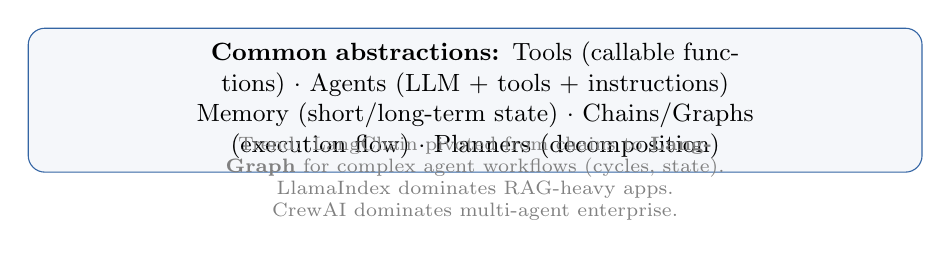
\begin{tikzpicture}
  \node[draw=popblue, fill=popblue!5, rounded corners=6pt, text width=11cm, align=center, inner sep=5pt, font=\small] at (0, 0) {
    \textbf{Common abstractions:} Tools (callable functions) $\cdot$ Agents (LLM + tools + instructions)\\
    Memory (short/long-term state) $\cdot$ Chains/Graphs (execution flow) $\cdot$ Planners (decomposition)
  };

  \node[font=\scriptsize, text=gray, text width=10cm, align=center] at (0, -1) {
    Trend: LangChain pivoted from chains to \textbf{LangGraph} for complex agent workflows (cycles, state).\\
    LlamaIndex dominates RAG-heavy apps. CrewAI dominates multi-agent enterprise.
  };
\end{tikzpicture}
\end{center}
\end{frame}

% ============================================================
% CODE AGENTS
% ============================================================
\begin{frame}
\frametitle{Code agents}

\begin{center}
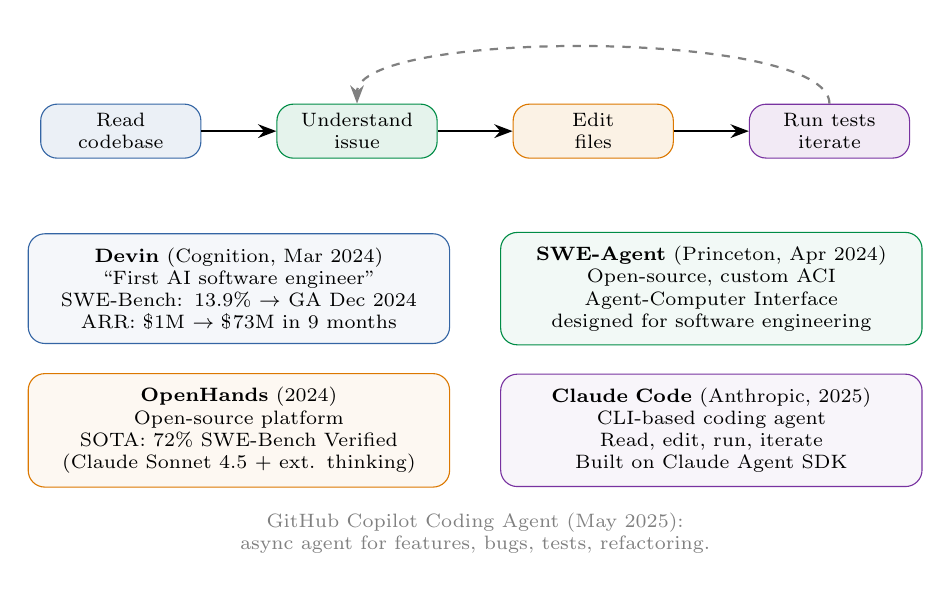
\begin{tikzpicture}
  % The loop
  \node[draw=popblue, fill=popblue!10, rounded corners=6pt, font=\scriptsize, text width=1.8cm, align=center] (read) at (-4.5, 2.5) {Read\\codebase};
  \node[draw=paramgreen, fill=paramgreen!10, rounded corners=6pt, font=\scriptsize, text width=1.8cm, align=center] (plan) at (-1.5, 2.5) {Understand\\issue};
  \node[draw=orange1, fill=orange1!10, rounded corners=6pt, font=\scriptsize, text width=1.8cm, align=center] (edit) at (1.5, 2.5) {Edit\\files};
  \node[draw=violet1, fill=violet1!10, rounded corners=6pt, font=\scriptsize, text width=1.8cm, align=center] (test) at (4.5, 2.5) {Run tests\\iterate};

  \draw[-Stealth, thick] (read) -- (plan);
  \draw[-Stealth, thick] (plan) -- (edit);
  \draw[-Stealth, thick] (edit) -- (test);
  \draw[-Stealth, thick, dashed, gray] (test) .. controls (4.5, 3.8) and (-1.5, 3.8) .. (plan);

  % Systems
  \node[draw=popblue, fill=popblue!5, rounded corners=6pt, text width=5cm, align=center, inner sep=5pt, font=\scriptsize] at (-3, 0.5) {
    \textbf{Devin} (Cognition, Mar 2024)\\
    ``First AI software engineer''\\
    SWE-Bench: 13.9\% $\to$ GA Dec 2024\\
    ARR: \$1M $\to$ \$73M in 9 months
  };

  \node[draw=paramgreen, fill=paramgreen!5, rounded corners=6pt, text width=5cm, align=center, inner sep=5pt, font=\scriptsize] at (3, 0.5) {
    \textbf{SWE-Agent} (Princeton, Apr 2024)\\
    Open-source, custom ACI\\
    Agent-Computer Interface\\
    designed for software engineering
  };

  \node[draw=orange1, fill=orange1!5, rounded corners=6pt, text width=5cm, align=center, inner sep=5pt, font=\scriptsize] at (-3, -1.3) {
    \textbf{OpenHands} (2024)\\
    Open-source platform\\
    SOTA: 72\% SWE-Bench Verified\\
    (Claude Sonnet 4.5 + ext. thinking)
  };

  \node[draw=violet1, fill=violet1!5, rounded corners=6pt, text width=5cm, align=center, inner sep=5pt, font=\scriptsize] at (3, -1.3) {
    \textbf{Claude Code} (Anthropic, 2025)\\
    CLI-based coding agent\\
    Read, edit, run, iterate\\
    Built on Claude Agent SDK
  };

  % GitHub
  \node[font=\scriptsize, text=gray, text width=10cm, align=center] at (0, -2.6) {
    GitHub Copilot Coding Agent (May 2025): async agent for features, bugs, tests, refactoring.
  };
\end{tikzpicture}
\end{center}
\end{frame}

% ============================================================
% SWE-BENCH EVOLUTION
% ============================================================
\begin{frame}
\frametitle{SWE-Bench: the code agent benchmark}
\vspace{-0.2cm}
\begin{center}
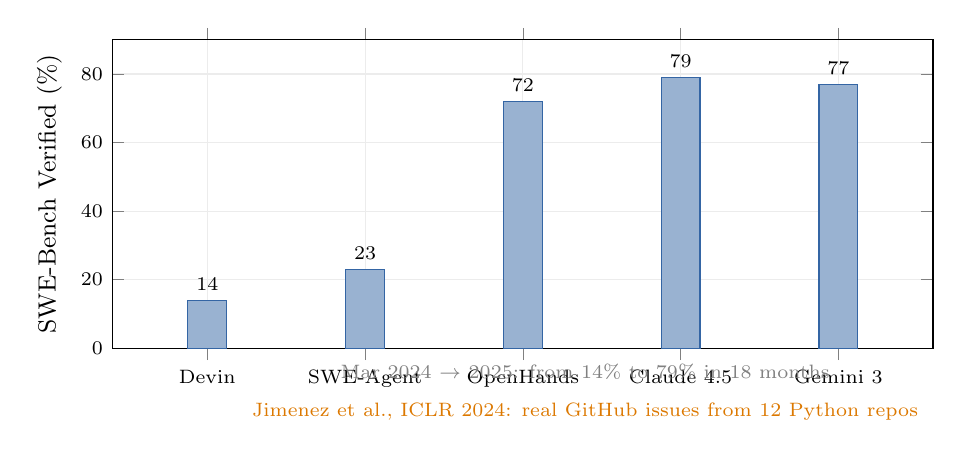
\begin{tikzpicture}
  \begin{axis}[
    width=12cm, height=5.5cm,
    ybar,
    bar width=14pt,
    ylabel={\small SWE-Bench Verified (\%)},
    symbolic x coords={Devin, SWE-Agent, OpenHands, Claude 4.5, Gemini 3},
    xtick=data,
    xticklabel style={font=\scriptsize},
    ymin=0, ymax=90,
    ytick={0, 20, 40, 60, 80},
    yticklabel style={font=\scriptsize},
    grid=major,
    grid style={gray!15},
    enlarge x limits=0.15,
    nodes near coords,
    every node near coord/.append style={font=\scriptsize},
  ]
    \addplot[fill=popblue!50, draw=popblue] coordinates {
      (Devin, 14) (SWE-Agent, 23) (OpenHands, 72) (Claude 4.5, 79) (Gemini 3, 77)
    };
  \end{axis}

  % Timeline annotation
  \node[font=\scriptsize, text=gray] at (6, -0.3) {Mar 2024 $\to$ 2025: from 14\% to 79\% in 18 months};
  \node[font=\scriptsize, text=orange1] at (6, -0.8) {Jimenez et al., ICLR 2024: real GitHub issues from 12 Python repos};
\end{tikzpicture}
\end{center}
\end{frame}

% ============================================================
% MCP: MODEL CONTEXT PROTOCOL
% ============================================================
\begin{frame}
\frametitle{MCP: Model Context Protocol}

\begin{center}
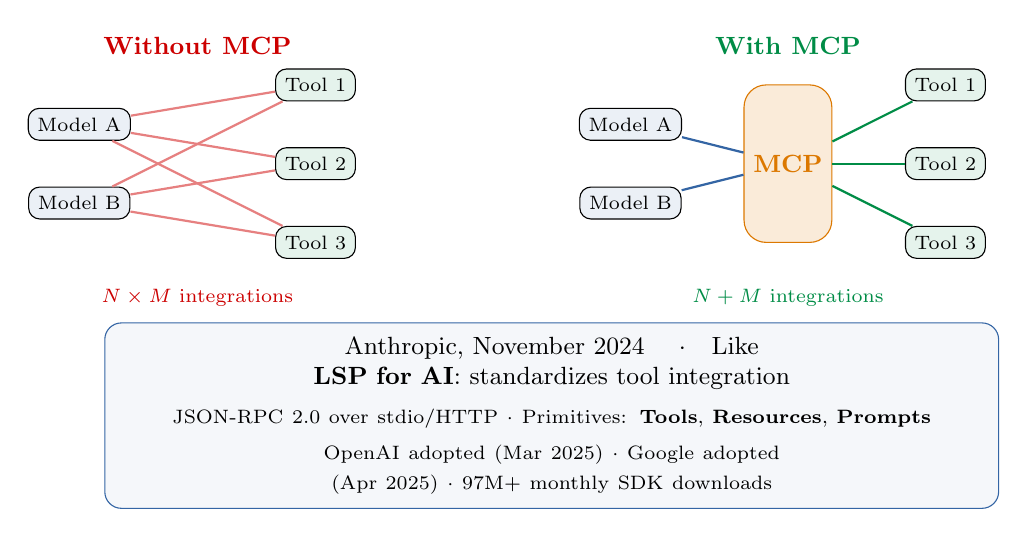
\begin{tikzpicture}
  % Without MCP
  \node[font=\small\bfseries, text=sampred] at (-4, 3.2) {Without MCP};
  \node[draw, rounded corners=4pt, fill=popblue!10, font=\scriptsize] (m1) at (-5.5, 2.2) {Model A};
  \node[draw, rounded corners=4pt, fill=popblue!10, font=\scriptsize] (m2) at (-5.5, 1.2) {Model B};
  \node[draw, rounded corners=4pt, fill=paramgreen!10, font=\scriptsize] (t1) at (-2.5, 2.7) {Tool 1};
  \node[draw, rounded corners=4pt, fill=paramgreen!10, font=\scriptsize] (t2) at (-2.5, 1.7) {Tool 2};
  \node[draw, rounded corners=4pt, fill=paramgreen!10, font=\scriptsize] (t3) at (-2.5, 0.7) {Tool 3};
  % N x M lines
  \draw[thick, sampred!50] (m1) -- (t1);
  \draw[thick, sampred!50] (m1) -- (t2);
  \draw[thick, sampred!50] (m1) -- (t3);
  \draw[thick, sampred!50] (m2) -- (t1);
  \draw[thick, sampred!50] (m2) -- (t2);
  \draw[thick, sampred!50] (m2) -- (t3);
  \node[font=\scriptsize, text=sampred] at (-4, 0) {$N \times M$ integrations};

  % With MCP
  \node[font=\small\bfseries, text=paramgreen] at (3.5, 3.2) {With MCP};
  \node[draw, rounded corners=4pt, fill=popblue!10, font=\scriptsize] (m3) at (1.5, 2.2) {Model A};
  \node[draw, rounded corners=4pt, fill=popblue!10, font=\scriptsize] (m4) at (1.5, 1.2) {Model B};
  \node[draw=orange1, fill=orange1!15, rounded corners=8pt, font=\small\bfseries, text=orange1, minimum height=2cm] (mcp) at (3.5, 1.7) {MCP};
  \node[draw, rounded corners=4pt, fill=paramgreen!10, font=\scriptsize] (t4) at (5.5, 2.7) {Tool 1};
  \node[draw, rounded corners=4pt, fill=paramgreen!10, font=\scriptsize] (t5) at (5.5, 1.7) {Tool 2};
  \node[draw, rounded corners=4pt, fill=paramgreen!10, font=\scriptsize] (t6) at (5.5, 0.7) {Tool 3};
  \draw[thick, popblue] (m3) -- (mcp);
  \draw[thick, popblue] (m4) -- (mcp);
  \draw[thick, paramgreen] (mcp) -- (t4);
  \draw[thick, paramgreen] (mcp) -- (t5);
  \draw[thick, paramgreen] (mcp) -- (t6);
  \node[font=\scriptsize, text=paramgreen] at (3.5, 0) {$N + M$ integrations};

  % Details
  \node[draw=popblue, fill=popblue!5, rounded corners=6pt, text width=11cm, align=center, inner sep=5pt, font=\small] at (0.5, -1.5) {
    Anthropic, November 2024 \quad$\cdot$\quad Like \textbf{LSP for AI}: standardizes tool integration\\[3pt]
    {\scriptsize JSON-RPC 2.0 over stdio/HTTP $\cdot$ Primitives: \textbf{Tools}, \textbf{Resources}, \textbf{Prompts}}\\[2pt]
    {\scriptsize OpenAI adopted (Mar 2025) $\cdot$ Google adopted (Apr 2025) $\cdot$ 97M+ monthly SDK downloads}
  };
\end{tikzpicture}
\end{center}
\end{frame}

% ============================================================
% CHALLENGES
% ============================================================
\begin{frame}
\frametitle{Challenges}

\begin{center}
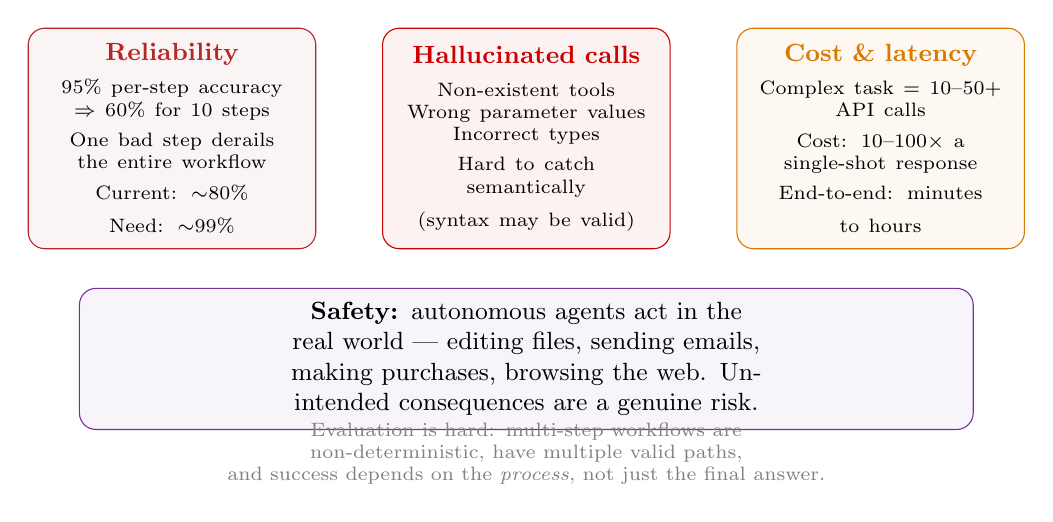
\begin{tikzpicture}
  % Reliability
  \node[draw=warnred, fill=warnred!5, rounded corners=6pt, text width=3.3cm, align=center, inner sep=5pt, minimum height=2.8cm] at (-4.5, 1.5) {
    {\small\bfseries\textcolor{warnred}{Reliability}}\\[4pt]
    {\scriptsize 95\% per-step accuracy\\$\Rightarrow$ 60\% for 10 steps\\[3pt]
    One bad step derails\\the entire workflow\\[3pt]
    Current: $\sim$80\%\\Need: $\sim$99\%}
  };

  % Hallucinated calls
  \node[draw=sampred, fill=sampred!5, rounded corners=6pt, text width=3.3cm, align=center, inner sep=5pt, minimum height=2.8cm] at (0, 1.5) {
    {\small\bfseries\textcolor{sampred}{Hallucinated calls}}\\[4pt]
    {\scriptsize Non-existent tools\\
    Wrong parameter values\\
    Incorrect types\\[3pt]
    Hard to catch semantically\\
    (syntax may be valid)}
  };

  % Cost & latency
  \node[draw=orange1, fill=orange1!5, rounded corners=6pt, text width=3.3cm, align=center, inner sep=5pt, minimum height=2.8cm] at (4.5, 1.5) {
    {\small\bfseries\textcolor{orange1}{Cost \& latency}}\\[4pt]
    {\scriptsize Complex task = 10--50+\\API calls\\[3pt]
    Cost: 10--100$\times$ a\\single-shot response\\[3pt]
    End-to-end: minutes\\to hours}
  };

  % Safety
  \node[draw=violet1, fill=violet1!5, rounded corners=6pt, text width=11cm, align=center, inner sep=5pt, font=\small] at (0, -1.3) {
    \textbf{Safety:} autonomous agents act in the real world --- editing files, sending emails,\\
    making purchases, browsing the web. Unintended consequences are a genuine risk.
  };

  % Evaluation
  \node[font=\scriptsize, text=gray, text width=10cm, align=center] at (0, -2.5) {
    Evaluation is hard: multi-step workflows are non-deterministic, have multiple valid paths,\\
    and success depends on the \textit{process}, not just the final answer.
  };
\end{tikzpicture}
\end{center}
\end{frame}

% ============================================================
% BENCHMARKS & EVALUATION
% ============================================================
\begin{frame}
\frametitle{Agent benchmarks}
\vspace{-0.2cm}
\renewcommand{\arraystretch}{1.3}
\begin{center}
{\small
\begin{tabular}{>{\bfseries}l l l l}
\hline
\textbf{Benchmark} & \textbf{What it measures} & \textbf{Scale} & \textbf{Key number} \\
\hline
SWE-Bench & Real GitHub issues & 2.3K tasks & Best: 79\% \\
AgentBench & 8 environments (OS, DB, ...) & 29 LLMs & Large open/closed gap \\
WebArena & Web browsing tasks & 812 tasks & 4 realistic domains \\
GAIA & General AI assistant & 466 Q & Human: 92\%, Best: 65\% \\
ToolBench & API tool use & 16K APIs & 49 categories \\
\hline
\end{tabular}
}
\end{center}

\vspace{0.3cm}
\begin{center}
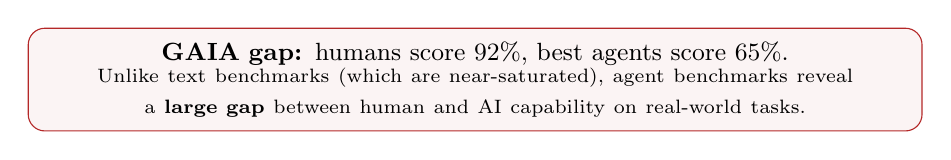
\begin{tikzpicture}
  \node[draw=warnred, fill=warnred!5, rounded corners=6pt, text width=11cm, align=center, inner sep=5pt, font=\small] at (0, 0) {
    \textbf{GAIA gap:} humans score 92\%, best agents score 65\%.\\
    {\scriptsize Unlike text benchmarks (which are near-saturated), agent benchmarks reveal\\
    a \textbf{large gap} between human and AI capability on real-world tasks.}
  };
\end{tikzpicture}
\end{center}
\end{frame}

% ============================================================
% COMPUTER USE AGENTS
% ============================================================
\begin{frame}
\frametitle{Computer use agents}

\begin{center}
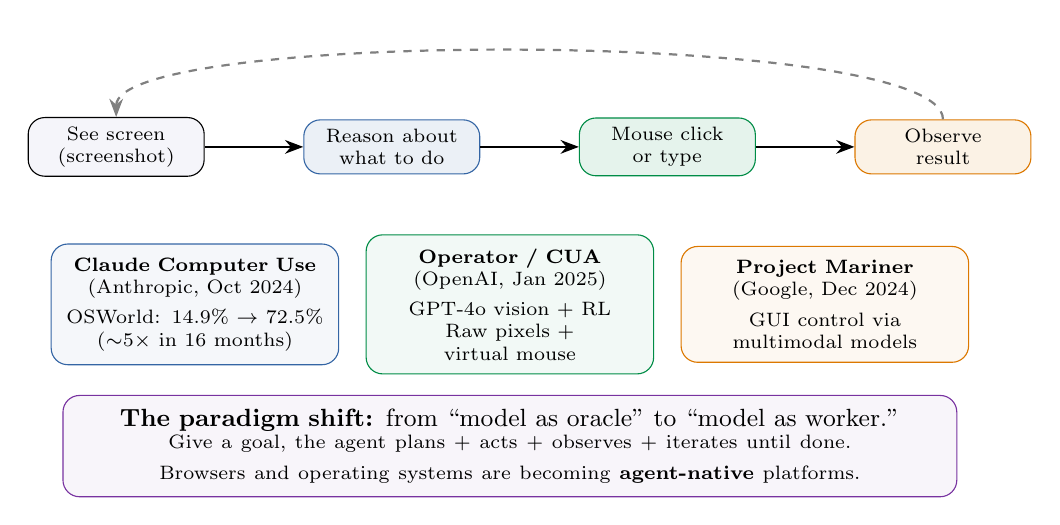
\begin{tikzpicture}
  % Pipeline
  \node[draw, rounded corners=6pt, fill=lightbg, font=\scriptsize, text width=2cm, align=center] (screen) at (-5, 2) {See screen\\(screenshot)};
  \node[draw=popblue, fill=popblue!10, rounded corners=6pt, font=\scriptsize, text width=2cm, align=center] (reason) at (-1.5, 2) {Reason about\\what to do};
  \node[draw=paramgreen, fill=paramgreen!10, rounded corners=6pt, font=\scriptsize, text width=2cm, align=center] (act) at (2, 2) {Mouse click\\or type};
  \node[draw=orange1, fill=orange1!10, rounded corners=6pt, font=\scriptsize, text width=2cm, align=center] (observe) at (5.5, 2) {Observe\\result};

  \draw[-Stealth, thick] (screen) -- (reason);
  \draw[-Stealth, thick] (reason) -- (act);
  \draw[-Stealth, thick] (act) -- (observe);
  \draw[-Stealth, thick, dashed, gray] (observe) .. controls (5.5, 3.5) and (-5, 3.5) .. (screen);

  % Systems
  \node[draw=popblue, fill=popblue!5, rounded corners=6pt, text width=3.3cm, align=center, inner sep=5pt, font=\scriptsize] at (-4, 0) {
    \textbf{Claude Computer Use}\\(Anthropic, Oct 2024)\\[3pt]
    OSWorld: 14.9\% $\to$ 72.5\%\\
    ($\sim$5$\times$ in 16 months)
  };

  \node[draw=paramgreen, fill=paramgreen!5, rounded corners=6pt, text width=3.3cm, align=center, inner sep=5pt, font=\scriptsize] at (0, 0) {
    \textbf{Operator / CUA}\\(OpenAI, Jan 2025)\\[3pt]
    GPT-4o vision + RL\\
    Raw pixels + virtual mouse
  };

  \node[draw=orange1, fill=orange1!5, rounded corners=6pt, text width=3.3cm, align=center, inner sep=5pt, font=\scriptsize] at (4, 0) {
    \textbf{Project Mariner}\\(Google, Dec 2024)\\[3pt]
    GUI control via\\multimodal models
  };

  % Bottom
  \node[draw=violet1, fill=violet1!5, rounded corners=6pt, text width=11cm, align=center, inner sep=5pt, font=\small] at (0, -1.8) {
    \textbf{The paradigm shift:} from ``model as oracle'' to ``model as worker.''\\
    {\scriptsize Give a goal, the agent plans + acts + observes + iterates until done.\\
    Browsers and operating systems are becoming \textbf{agent-native} platforms.}
  };
\end{tikzpicture}
\end{center}
\end{frame}

% ============================================================
% PRACTICAL GUIDE
% ============================================================
\begin{frame}
\frametitle{Practical guide}

\begin{center}
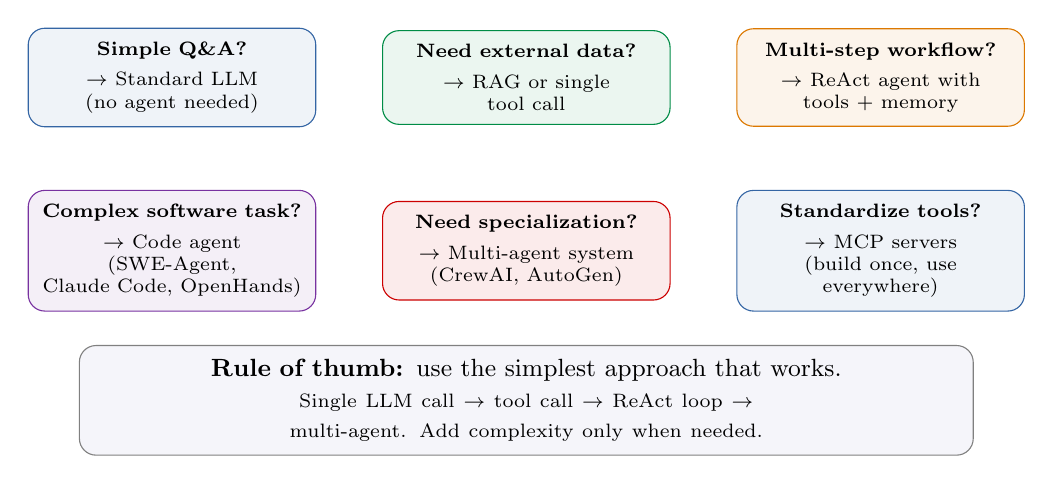
\begin{tikzpicture}
  % Decision boxes
  \node[draw=popblue, fill=popblue!8, rounded corners=6pt, text width=3.3cm, align=center, inner sep=5pt, font=\scriptsize] at (-4.5, 2.5) {
    \textbf{Simple Q\&A?}\\[3pt]
    $\to$ Standard LLM\\(no agent needed)
  };

  \node[draw=paramgreen, fill=paramgreen!8, rounded corners=6pt, text width=3.3cm, align=center, inner sep=5pt, font=\scriptsize] at (0, 2.5) {
    \textbf{Need external data?}\\[3pt]
    $\to$ RAG or single\\tool call
  };

  \node[draw=orange1, fill=orange1!8, rounded corners=6pt, text width=3.3cm, align=center, inner sep=5pt, font=\scriptsize] at (4.5, 2.5) {
    \textbf{Multi-step workflow?}\\[3pt]
    $\to$ ReAct agent with\\tools + memory
  };

  \node[draw=violet1, fill=violet1!8, rounded corners=6pt, text width=3.3cm, align=center, inner sep=5pt, font=\scriptsize] at (-4.5, 0.3) {
    \textbf{Complex software task?}\\[3pt]
    $\to$ Code agent (SWE-Agent,\\Claude Code, OpenHands)
  };

  \node[draw=sampred, fill=sampred!8, rounded corners=6pt, text width=3.3cm, align=center, inner sep=5pt, font=\scriptsize] at (0, 0.3) {
    \textbf{Need specialization?}\\[3pt]
    $\to$ Multi-agent system\\(CrewAI, AutoGen)
  };

  \node[draw=popblue, fill=popblue!8, rounded corners=6pt, text width=3.3cm, align=center, inner sep=5pt, font=\scriptsize] at (4.5, 0.3) {
    \textbf{Standardize tools?}\\[3pt]
    $\to$ MCP servers\\(build once, use everywhere)
  };

  % Bottom
  \node[draw=gray, fill=lightbg, rounded corners=6pt, text width=11cm, align=center, inner sep=5pt, font=\small] at (0, -1.6) {
    \textbf{Rule of thumb:} use the simplest approach that works.\\
    {\scriptsize Single LLM call $\to$ tool call $\to$ ReAct loop $\to$ multi-agent. Add complexity only when needed.}
  };
\end{tikzpicture}
\end{center}
\end{frame}

% ============================================================
% FURTHER READING
% ============================================================
\begin{frame}
\frametitle{Further reading}
\vspace{-0.3cm}
\begin{center}
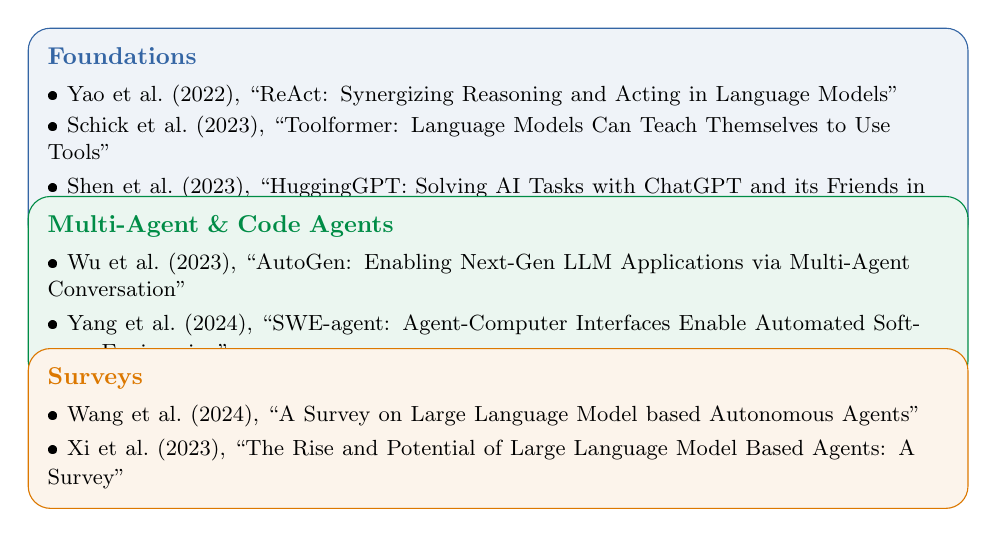
\begin{tikzpicture}[scale=0.88, transform shape]
  \node[draw=popblue, fill=popblue!8, rounded corners=8pt, text width=13cm, align=left, inner sep=8pt] at (0, 2.5) {
    \textbf{\textcolor{popblue}{Foundations}}\\[4pt]
    {\small
    \textbullet~Yao et al.\ (2022), ``ReAct: Synergizing Reasoning and Acting in Language Models''\\[2pt]
    \textbullet~Schick et al.\ (2023), ``Toolformer: Language Models Can Teach Themselves to Use Tools''\\[2pt]
    \textbullet~Shen et al.\ (2023), ``HuggingGPT: Solving AI Tasks with ChatGPT and its Friends in HuggingFace''
    }
  };
  \node[draw=paramgreen, fill=paramgreen!8, rounded corners=8pt, text width=13cm, align=left, inner sep=8pt] at (0, 0.3) {
    \textbf{\textcolor{paramgreen}{Multi-Agent \& Code Agents}}\\[4pt]
    {\small
    \textbullet~Wu et al.\ (2023), ``AutoGen: Enabling Next-Gen LLM Applications via Multi-Agent Conversation''\\[2pt]
    \textbullet~Yang et al.\ (2024), ``SWE-agent: Agent-Computer Interfaces Enable Automated Software Engineering''
    }
  };
  \node[draw=orange1, fill=orange1!8, rounded corners=8pt, text width=13cm, align=left, inner sep=8pt] at (0, -1.7) {
    \textbf{\textcolor{orange1}{Surveys}}\\[4pt]
    {\small
    \textbullet~Wang et al.\ (2024), ``A Survey on Large Language Model based Autonomous Agents''\\[2pt]
    \textbullet~Xi et al.\ (2023), ``The Rise and Potential of Large Language Model Based Agents: A Survey''
    }
  };
\end{tikzpicture}
\end{center}
\end{frame}

% ============================================================
% QUESTIONS
% ============================================================
\begin{frame}
\begin{center}
\vspace{2cm}
{\Huge \textcolor{popblue}{Questions?}}

\vspace{1cm}
{\normalsize All DL4NLP topics complete!}
\end{center}
\end{frame}

\end{document}
